%-------------------------------------
\begin{frame}
\frametitle{The ``Active Stance''}
\begin{columns}[c] % The "c" option specifies centered vertical alignment while the "t" option is used for top vertical alignment

\column{.2\textwidth} % Left column and width
%	\begin{figure}
	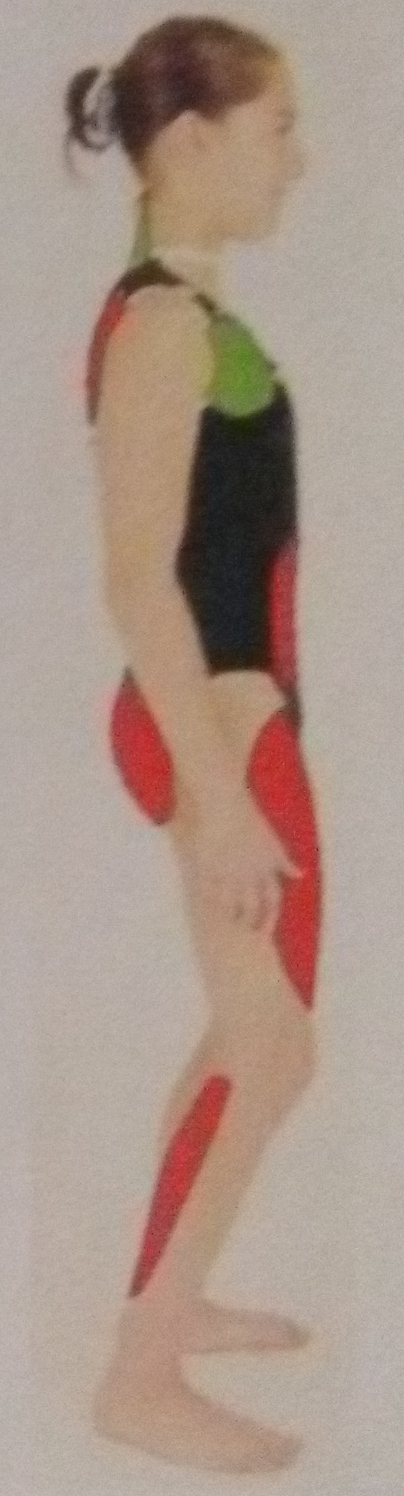
\includegraphics[width=0.85\linewidth]{AS6.png} % 15 %, 10% = 7.2
%	\end{figure}

\column{.6\textwidth} % Left column and width



This exercise helps to train a \structure{stable and conscious posture} and is best controlled in front of a mirror. It's best to get in the habit of adapt this position as much as possible. This strengthens and stretches muscle groups, which are important for a good posture.

This picture shows the especially \structure{active} (red) and the \structure{stretched} (green) muscle groups.
\end{columns}
\end{frame}
%-------------------------------------
\begin{frame}
\frametitle{2) Bend your knees slightly}
\begin{columns}[c] % The "c" option specifies centered vertical alignment while the "t" option is used for top vertical alignment

\column{.2\textwidth} % Left column and width
%	\begin{figure}
	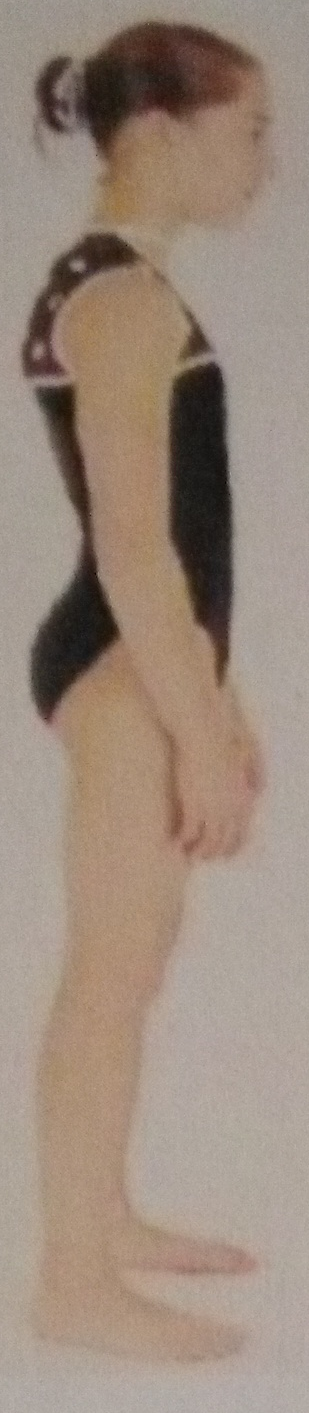
\includegraphics[width=0.7\linewidth]{AS1.png}
%	\end{figure}

\column{.4\textwidth} % Left column and width

Starting with the starting position (1), the \structure{knees} get slightly \structure{bend}. The \structure{weight} stays \structure{evenly distributed} on your feet, no leaning backwards.

The \structure{tension in the thighs} should be well noticeable.

\column{.24\textwidth} % Left column and width
%	\begin{figure}
	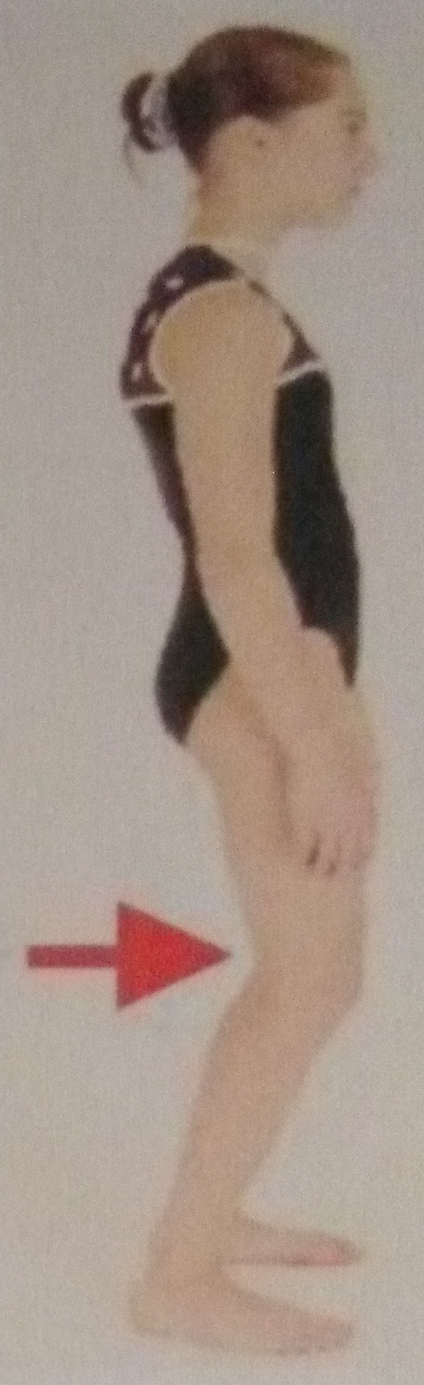
\includegraphics[width=0.81\linewidth]{AS2.png}
%	\end{figure}
\end{columns}
\end{frame}
%-------------------------------------
\begin{frame}
\frametitle{3) The most difficult part}
\begin{columns}[c] % The "c" option specifies centered vertical alignment while the "t" option is used for top vertical alignment

\column{.28\textwidth} % Left column and width
%	\begin{figure}
	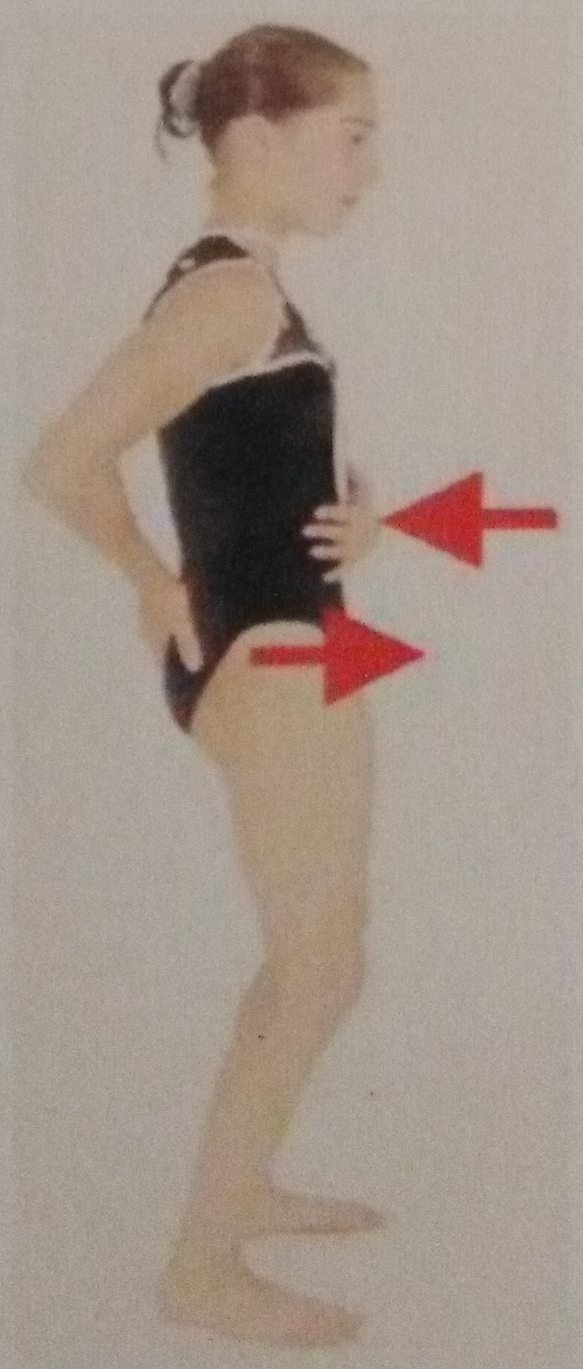
\includegraphics[width=.95\linewidth]{AS3.png}
%	\end{figure}

\column{.4\textwidth} % Left column and width

\structure{Tense up your buttocks and the abdominal muscles}. Push the \structure{hip slightly forward}. That causes the hip bone to rotate counter clockwise around the hip joint as axis. The hollow back should disappear. \structure{Hold the tension} in your buttocks.


\column{.33\textwidth} % Left column and width
%	\begin{figure}
	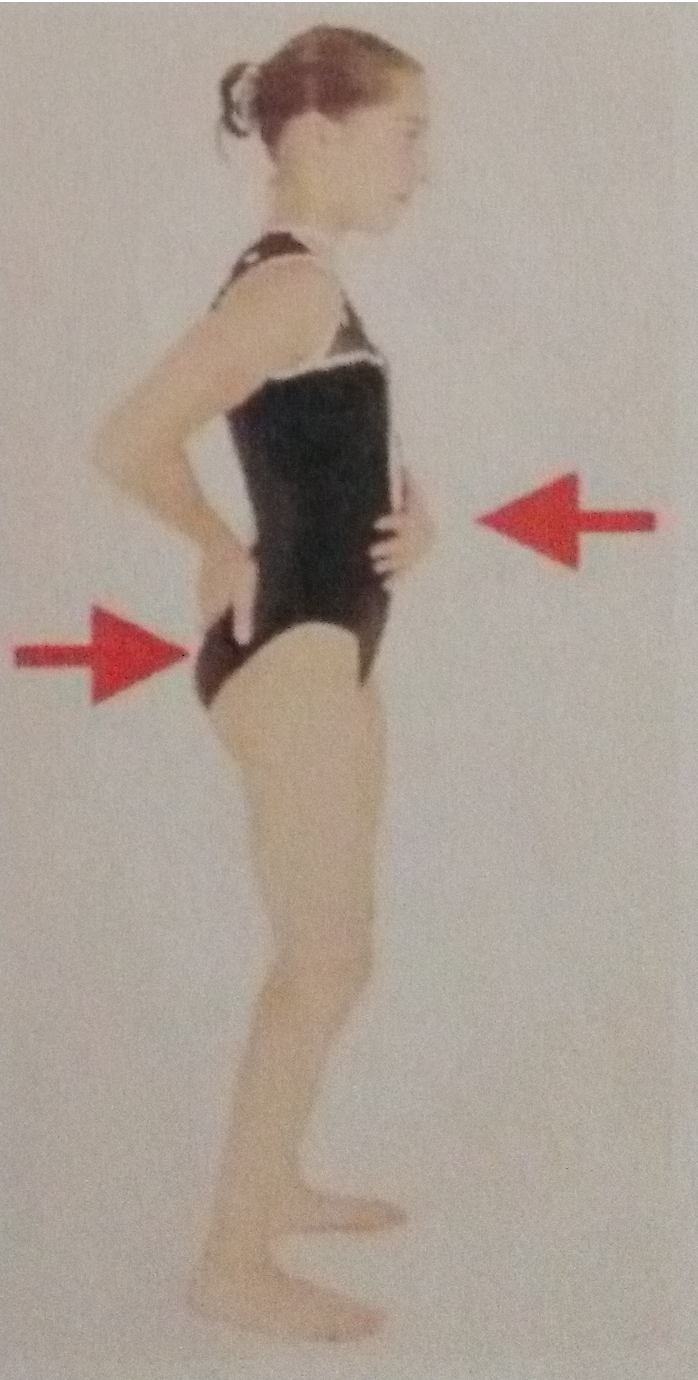
\includegraphics[width=.95\linewidth]{AS4.png}
%	\end{figure}
\end{columns}
\end{frame}
%-------------------------------------
\begin{frame}
\frametitle{4) Push the shoulders back}
\begin{columns}[c] % The "c" option specifies centered vertical alignment while the "t" option is used for top vertical alignment

\column{.3\textwidth} % Left column and width
%	\begin{figure}
	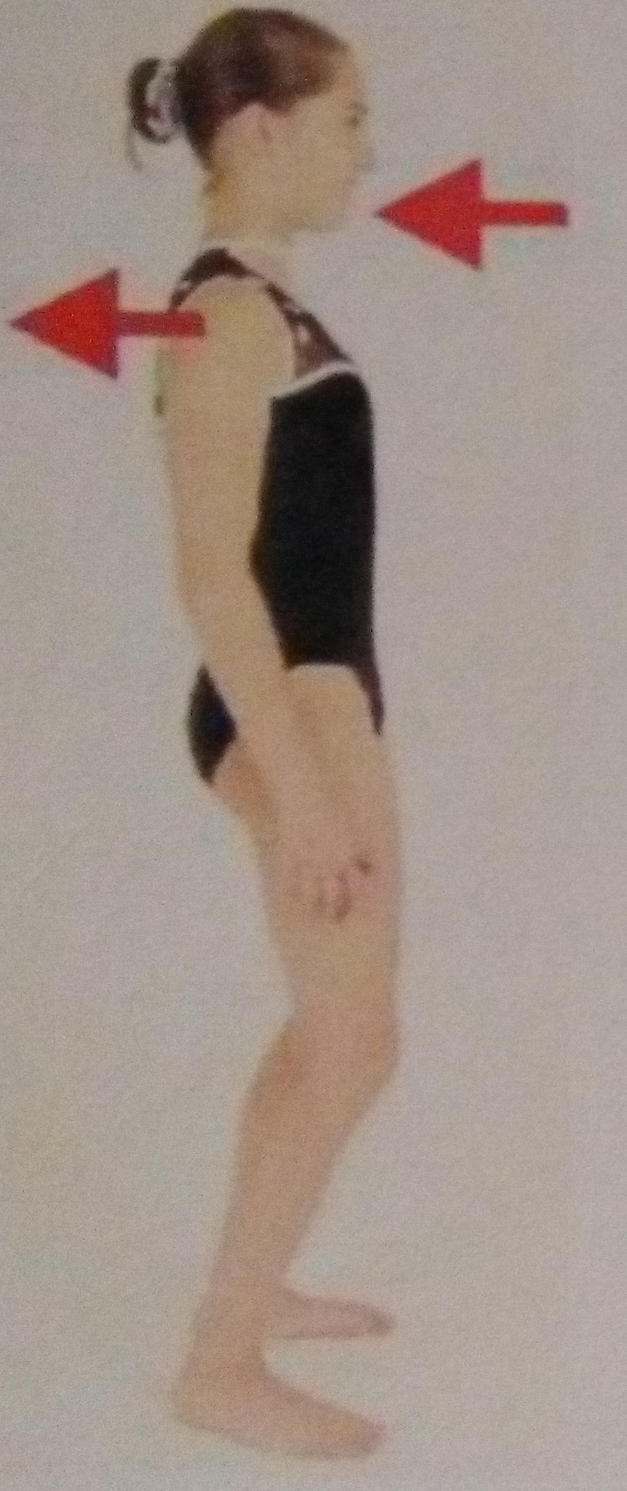
\includegraphics[width=.89\linewidth]{AS5.png}
%	\end{figure}

\column{.4\textwidth} % Left column and width

\structure{Push your chin back} (make a ``double chin''). This end position should be \structure{hold as long as possible}. 

The figure on the right shows the \structure{final position}, with the active (red) and stretched muscle groups.

\vspace{1cm}
Back to \href{run:./Exercises.pdf}{\underline{exercises}}.

\column{.2\textwidth} % Left column and width
%	\begin{figure}
	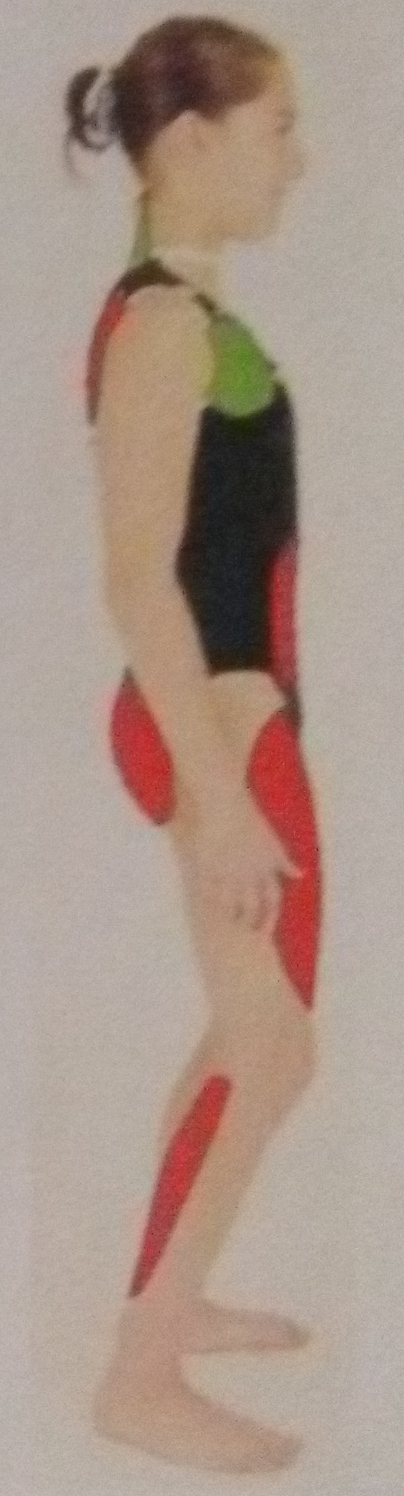
\includegraphics[width=.84\linewidth]{AS6.png}
%	\end{figure}
\end{columns}
\end{frame}